
% 默认配方: xelatex -> biber -> xelatex -> xelatex
% 与 HW1 报告保持同一 elegantpaper 样式。
\ifdefined\ELEGANTBibTeXBackend
  \PassOptionsToClass{bibtex}{elegantpaper}
\fi
\documentclass[lang=cn,a4paper,newtx,code=minted]{elegantpaper}

\usepackage{tabularx}
\usepackage{float}
\usepackage[section]{placeins}
\usepackage{array}
\usepackage{siunitx}
\usepackage{subcaption}
\usepackage{makecell}
\usepackage{enumitem}
\usepackage{xurl}
\graphicspath{{pic/}{../pic/}}

\renewcommand{\topfraction}{0.9}
\renewcommand{\textfraction}{0.07}
\renewcommand{\floatpagefraction}{0.8}
\setlength{\textfloatsep}{10pt plus 2pt minus 2pt}
\setlength{\floatsep}{8pt plus 2pt minus 2pt}
\setlength{\intextsep}{8pt plus 2pt minus 2pt}
\captionsetup[table]{font=small,labelfont=bf,skip=4pt}
\captionsetup[figure]{font=small,labelfont=bf,skip=3pt}
\setlength{\tabcolsep}{4pt}
\renewcommand{\arraystretch}{1.08}
\sisetup{detect-all,detect-weight=true,detect-family=true,group-digits=false,table-number-alignment=center,table-text-alignment=center}
\newcolumntype{L}[1]{>{\raggedright\arraybackslash}p{#1}}
\newcolumntype{C}[1]{>{\centering\arraybackslash}p{#1}}
\newcolumntype{R}[1]{>{\raggedleft\arraybackslash}p{#1}}

\title{CS60003 期中作业实验报告：分类、检测跟踪与语义分割}
\author{夏商周 \quad 25210980114 \quad Task1 \\ 杨智超 \quad 25210980124 \quad Task2 \\ 杨晨 \quad 25210980120 \quad Task3}
\institute{\href{https://github.com/YangChen-pro/CS60003}{代码仓库}\quad|\quad\href{https://modelscope.cn/models/youngchen/CS60003/}{模型仓库}}
\date{\zhdate{2026/05/17}}

\begin{document}
\maketitle

\begin{abstract}
本报告记录 CS60003 期中作业三个任务的实现与实验结果。Task 1 在 102 Category Flower Dataset 上微调 ImageNet 预训练卷积网络，完成 ResNet-18 baseline、超参数对比、随机初始化消融和 SE 注意力结构对比，并额外用 ConvNeXt-Tiny 获得当前最高 test accuracy 96.08\%。Task 2 在 Road Vehicle Images Dataset 上训练 YOLOv8s 检测器，最佳 epoch 的 mAP50 为 0.5150、mAP50--95 为 0.2854，并结合 ByteTrack、轨迹重连和越线判断完成 10--30 秒交通视频的多目标跟踪与计数。Task 3 在 Stanford Background Dataset 上从零手写 U-Net 与 Dice Loss，比较 Cross-Entropy、Dice 与 CE+Dice 三组损失，并在不使用预训练和现成分割模型的约束下继续优化到 validation mIoU 70.1053\%。
\keywords{Flowers102，YOLOv8，ByteTrack，ResNet 微调，U-Net，Dice Loss，SwanLab}
\end{abstract}

\section{实验总览与提交资源}

本次作业包含三个任务。代码统一提交至公开 \href{https://github.com/YangChen-pro/CS60003/tree/main/hw2}{GitHub 仓库}，训练权重与关键实验产物统一发布到 ModelScope \href{https://www.modelscope.cn/models/youngchen/CS60003/tree/master/hw2}{模型仓库}，按 \texttt{hw2/task1/}、\texttt{hw2/task2/} 与 \texttt{hw2/task3/} 子目录组织。

\begin{table}[!htbp]
\centering
\small
\caption{当前报告覆盖范围与交付物}
\label{tab:overview}
\begin{tabular}{@{}L{0.17\linewidth}L{0.43\linewidth}L{0.31\linewidth}@{}}
\toprule
任务 & 当前状态 & 主要交付物 \\
\midrule
Task 1 & 已完成 Flowers102 分类实验、SwanLab 记录和 ModelScope 上传 & \href{https://www.modelscope.cn/models/youngchen/CS60003/tree/master/hw2/task1}{仓库}：\texttt{hw2/task1/.../best.pt} \\
Task 2 & 已完成车辆检测训练、视频多目标跟踪、遮挡分析和越线计数 & \href{https://www.modelscope.cn/models/youngchen/CS60003/tree/master/hw2/task2}{仓库}：\texttt{hw2/task2/.../best.pt} \\
Task 3 & 已完成 Stanford Background 分割实验、SwanLab 记录和 ModelScope 上传 & \href{https://www.modelscope.cn/models/youngchen/CS60003/tree/master/hw2/task3}{仓库}：\texttt{hw2/task3/.../best.pt} \\
\bottomrule
\end{tabular}
\end{table}

报告中的训练曲线来自 SwanLab 实验记录或同一训练历史导出的图片，已随报告图片目录保存，正文不公开私有实验页面。为保证材料可复现，Task 2 除检测权重外还保留 \texttt{metrics.json}、\texttt{history.csv}、跟踪配置和 30/60 fps 两组计数摘要。

\section{Task 1：ImageNet 预训练卷积网络的 Flowers102 微调}

\subsection{任务要求与实现概述}

Task 1 要求在 102 Category Flower Dataset 上修改 CNN 输出层作为 baseline，使用 ImageNet 预训练参数初始化，采用较小学习率微调 backbone、较大学习率训练新分类头，并观察训练步数、学习率等超参数的影响。同时，还需要比较随机初始化与预训练初始化，并在 baseline 基础上加入注意力模块或使用轻量 Transformer 进行对比。

实现位于 \texttt{hw2/task1/}。数据读取严格使用官方 \texttt{setid.mat}：训练集、验证集和测试集分别为 1020、1020 和 6149 张。模型构建使用 \texttt{torchvision} 中的 ResNet-18/34/50、EfficientNet-B0 与 ConvNeXt-Tiny；其中 baseline 与作业主线围绕 ResNet-18/34 展开，ConvNeXt-Tiny 只作为额外提升模型报告。优化器支持 SGD 与 AdamW，训练过程中按验证集 accuracy 保存最佳 checkpoint。

\subsection{模型与训练设置}

Baseline 使用 ImageNet 预训练 ResNet-18，将原分类层替换为 102 类线性层。参数组分为 backbone 和 classifier 两部分，baseline 的 backbone learning rate 为 $1\times10^{-4}$，classifier learning rate 为 $1\times10^{-3}$。随机初始化消融只把 \texttt{pretrained} 置为 \texttt{false}，其余训练预算保持可比。注意力模型采用手写 SE block 插入 ResNet BasicBlock 的第二个 batch normalization 之后、残差相加之前。

\begin{table}[!htbp]
\centering
\small
\caption{Task 1 数据与 baseline 训练配置}
\label{tab:task1-config}
\begin{tabular}{@{}L{0.26\linewidth}L{0.56\linewidth}@{}}
\toprule
项目 & 配置 \\
\midrule
数据集 & Oxford 102 Category Flower Dataset，102 类 \\
官方划分 & train 1020 / val 1020 / test 6149 \\
输入尺寸 & $224\times224$；最终高分实验使用相同尺寸 \\
Baseline & ImageNet 预训练 ResNet-18，替换 102 类输出层 \\
优化器 & SGD，momentum 0.9，cosine scheduler \\
学习率 & backbone $1\times10^{-4}$，classifier $1\times10^{-3}$ \\
训练轮数 & baseline 40 epochs；优化实验最高 71 epochs \\
Batch size & baseline 64；ConvNeXt-Tiny 最终实验 32 \\
正则与损失 & baseline Cross-Entropy + weight decay $10^{-4}$；最终实验使用 AdamW、weight decay 0.05 和 label smoothing 0.05 \\
增强策略 & baseline 使用标准随机裁剪/翻转；最终实验加入 RandAugment、RandomErasing 和 horizontal-flip TTA \\
评价指标 & validation accuracy 选模，test accuracy 报告最终泛化结果 \\
\bottomrule
\end{tabular}
\end{table}

\subsection{Baseline、消融与超参数对比}

表 \ref{tab:task1-results} 汇总了报告必要实验。Baseline test accuracy 为 68.19\%。随机初始化 ResNet-18 在相同训练预算下只有 15.71\%，说明 ImageNet 预训练对小样本细粒度花卉分类至关重要。低学习率和短训练轮数均明显欠拟合；加入 label smoothing 后，ResNet-18 test accuracy 提升到 76.89\%。SE-ResNet-18 虽然满足注意力结构要求，但当前设置下没有超过 baseline；这只能说明当前 SE 插入位置和训练策略未带来收益，不能推出注意力机制总体无效。ResNet-34 强增强作为 ResNet 系列优化代表达到 81.72\%。最终额外优化模型 ConvNeXt-Tiny 达到 96.08\%，用于最终模型提交。图 \ref{fig:task1-curves} 展示了 baseline 与最终模型的训练曲线差异，ConvNeXt-Tiny 的验证 accuracy 更快进入高位且后期波动更小。

\begin{table}[!htbp]
\centering
\small
\caption{Task 1 关键实验结果（粗体为最佳，下划线为次优）}
\label{tab:task1-results}
\begin{tabular}{@{}L{0.32\linewidth}L{0.25\linewidth}C{0.14\linewidth}C{0.14\linewidth}@{}}
\toprule
实验 & 作用 & {Best val acc} & {Test acc} \\
\midrule
Baseline ResNet-18 & 预训练 baseline & 0.7186 & 0.6819 \\
低学习率 ResNet-18 & 学习率消融 & 0.4873 & 0.4506 \\
较短训练 ResNet-18 & 训练步数消融 & 0.5725 & 0.5307 \\
随机初始化 ResNet-18 & 预训练消融 & 0.1794 & 0.1571 \\
SE-ResNet-18 & 注意力机制对比 & 0.4500 & 0.4245 \\
ResNet-18 label smoothing & 超参数优化 & 0.7745 & 0.7689 \\
ResNet-34 强增强 & ResNet 系列优化 & \underline{0.8284} & \underline{0.8172} \\
ConvNeXt-Tiny 优化 & 最终额外提升模型 & \textbf{0.9784} & \textbf{0.9608} \\
\bottomrule
\end{tabular}
\end{table}

\begin{figure}[!htbp]
\centering
\begin{subfigure}{0.82\textwidth}
  \centering
  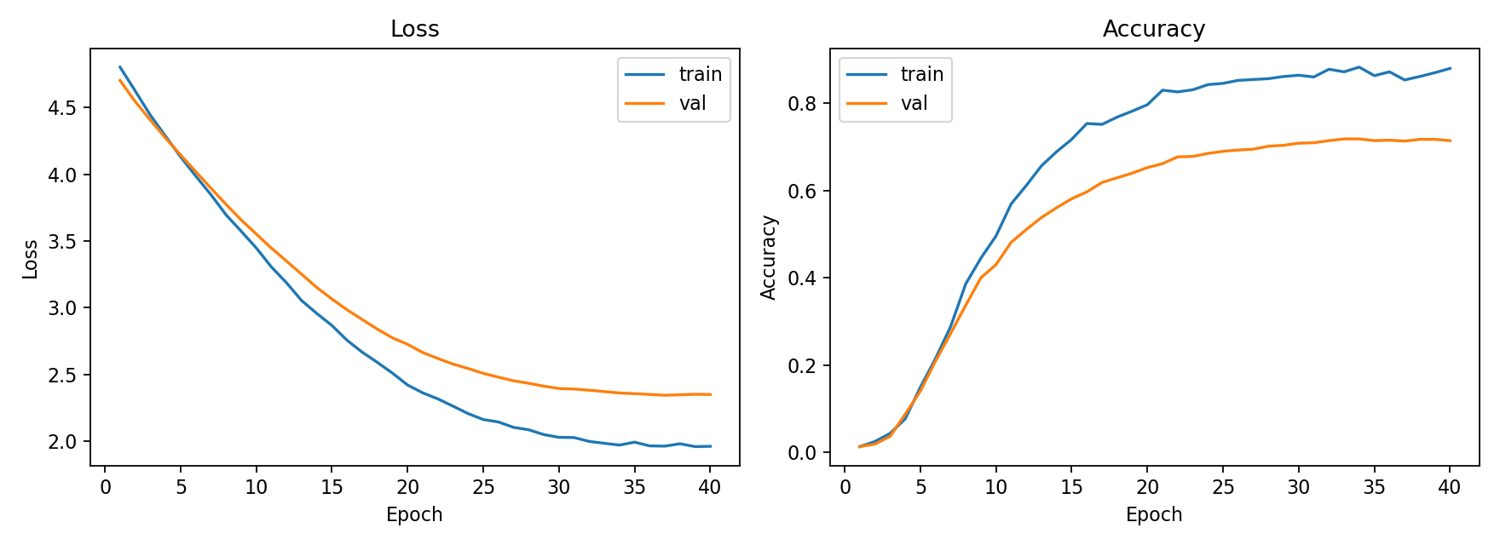
\includegraphics[width=\linewidth]{task1_baseline_curves.jpg}
  \caption{Baseline ResNet-18}
\end{subfigure}
\vspace{4pt}

\begin{subfigure}{0.82\textwidth}
  \centering
  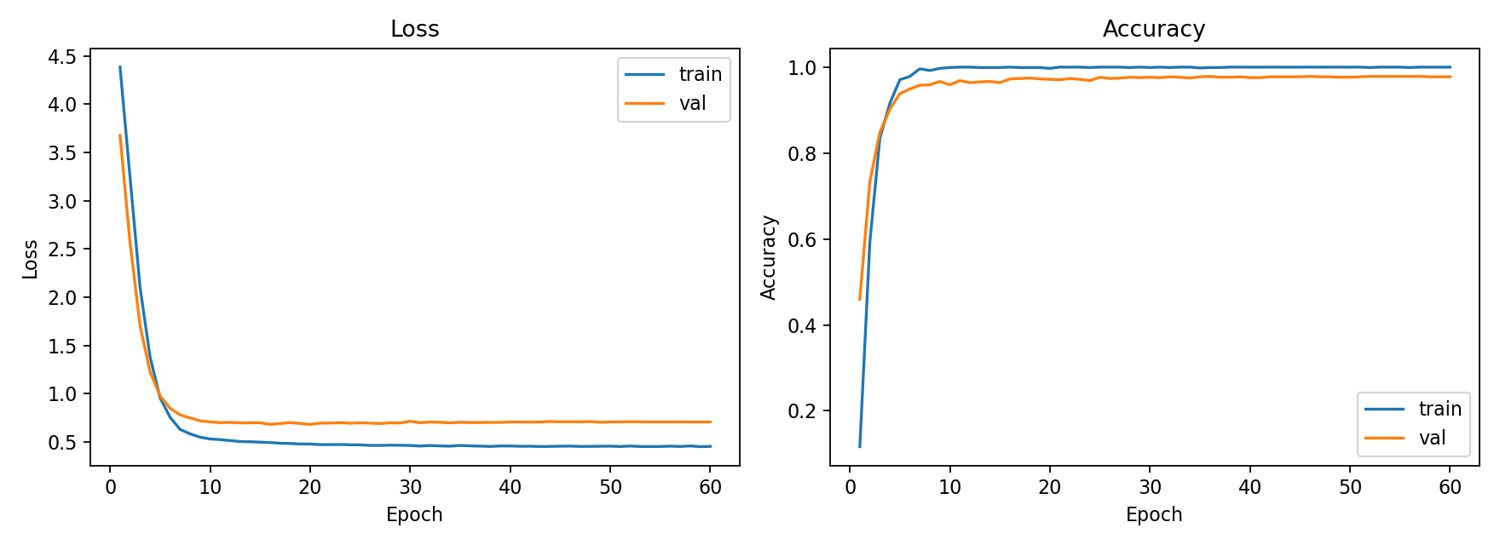
\includegraphics[width=\linewidth]{task1_convnext_curves.jpg}
  \caption{ConvNeXt-Tiny 最终优化}
\end{subfigure}
\caption{Task 1 SwanLab 曲线。横轴为 Epoch，纵轴为 Loss 与 Accuracy。}
\label{fig:task1-curves}
\end{figure}

\subsection{Task 1 小结}

Task 1 的合规主线由 ResNet-18 baseline、学习率/epoch 超参数对比、随机初始化消融和 SE 注意力对比构成。最终提交模型选择 ConvNeXt-Tiny，是在完成主线要求后额外加入的强 ImageNet 预训练 backbone。ConvNeXt-Tiny 的优势主要来自更强的 ImageNet 表征、现代卷积结构、AdamW 正则化和更充分的数据增强；注意力机制实验仍以 SE-ResNet-18 为依据。

\section{Task 2：Road Vehicle 目标检测与多目标跟踪}

\subsection{任务要求与实现概述}

Task 2 围绕交通场景中的车辆检测与多目标跟踪展开。作业要求先在 Road Vehicle Images Dataset 上微调 YOLOv8 或同类现代单阶段检测器，得到自己的检测权重；再选取一段 10--30 秒的测试视频，逐帧输出 bounding box、类别和 tracking ID，并进一步分析遮挡场景下的 ID 稳定性，最后根据虚拟线完成越线计数。

实现位于 \texttt{hw2/task2/}。整体流程先训练 YOLOv8s 检测器，得到逐帧类别、置信度和边界框；随后将检测结果输入 ByteTrack 维护轨迹，并在 raw track id 之上增加一层 display id，用于视频可视化和越线计数。检测阶段只解决单帧定位问题，跟踪阶段再利用目标中心点的时间连续性判断 ID 延续与越线事件。由于测试视频中存在小二轮车、密集交汇和短时遮挡，最终计数还加入了轨迹重连、短时丢失目标预测和重复越线去重。

\subsection{检测模型与训练设置}

检测模型采用 YOLOv8s。该模型仍属于单阶段检测框架，推理速度适合视频流处理，同时比 YOLOv8n 具备更强的特征表达能力，对远处车辆和二轮车等小目标更稳。数据集使用 Road Vehicle Images Dataset 的 YOLO 标注格式，共 21 个类别，训练集和验证集分别为 2704 与 300 张图像。

\begin{table}[!htbp]
\centering
\small
\caption{Task 2 检测训练配置}
\label{tab:task2-config}
\begin{tabular}{@{}L{0.28\linewidth}L{0.56\linewidth}@{}}
\toprule
项目 & 配置 \\
\midrule
数据集 & Road Vehicle Images Dataset，YOLO 标注格式，21 类 \\
划分 & train 2704 / valid 300 \\
检测模型 & YOLOv8s，COCO 预训练权重初始化后微调检测头与 backbone \\
输入尺寸 & $640\times640$ \\
训练轮数 & 50 epochs，保存验证集 mAP 最优 checkpoint \\
Batch size & 16 \\
优化器 & AdamW，初始学习率 0.001，最终学习率比例 0.01，warmup 3 epochs \\
混合精度 & AMP 开启 \\
跟踪阈值 & 推理置信度 0.1，ByteTrack \texttt{track\_buffer}=120 \\
\bottomrule
\end{tabular}
\end{table}

\subsection{检测训练结果}

表 \ref{tab:task2-det-result} 给出检测模型的主要指标。最佳 checkpoint 出现在 epoch 38，mAP50 为 0.5150，mAP50--95 为 0.2854。该结果能够支撑后续视频跟踪，但也说明检测框质量仍有提升空间：在较宽松 IoU 阈值下模型可以较稳定地发现车辆，而在更严格阈值下，小目标、遮挡目标和边界不清晰目标仍容易产生定位误差。

\begin{table}[!htbp]
\centering
\small
\caption{Task 2 YOLOv8s 检测结果}
\label{tab:task2-det-result}
\begin{tabular}{@{}L{0.26\linewidth}C{0.18\linewidth}C{0.18\linewidth}C{0.18\linewidth}@{}}
\toprule
模型 & Best epoch & mAP50 & mAP50--95 \\
\midrule
YOLOv8s baseline & 38 & 0.5150 & 0.2854 \\
\bottomrule
\end{tabular}
\end{table}

\begin{figure}[!htbp]
\centering
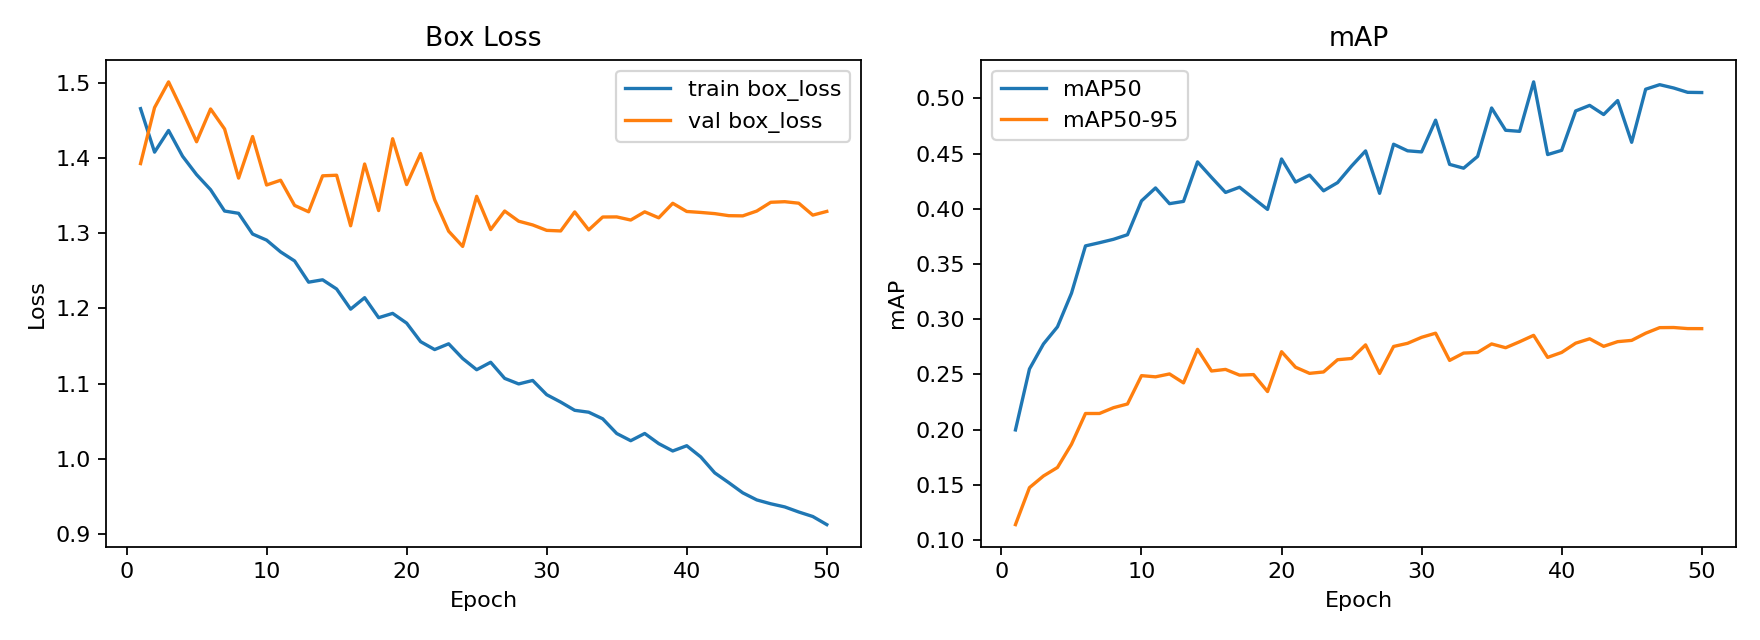
\includegraphics[width=0.95\textwidth]{task2_yolov8s_curves.png}
\caption{Task 2 YOLOv8s 训练曲线。左图为 box loss，右图为 mAP50 与 mAP50--95。}
\label{fig:task2-curves}
\end{figure}

图 \ref{fig:task2-curves} 中训练 box loss 持续下降，说明边界框回归在训练过程中稳定收敛。验证 box loss 的波动更明显，主要来自道路场景中尺度差异很大的车辆、远处小目标以及局部遮挡目标。mAP50 在训练中后段逐步提升到约 0.5，mAP50--95 的增幅相对有限，说明模型已经具备可用的召回和粗定位能力，但高精度框定位仍是后续跟踪的主要误差来源。基于这一点，视频推理阶段没有使用过高置信度阈值，而是保留部分低置信度检测交给 ByteTrack 进行时序筛选。

\subsection{视频跟踪与越线计数}

视频推理阶段分别处理 30 fps 与 60 fps 两个版本。每一帧先由训练好的 YOLOv8s 产生检测框，再由 ByteTrack 根据框位置、置信度和运动预测生成 raw track id。输出视频中，每个目标均显示 bounding box、类别、display id 与置信度，例如 \texttt{motorbike \#11 0.52}。display id 不直接等同于 ByteTrack 的 raw id，而是在短时遮挡或漏检后尝试延续同一目标身份，避免视频中频繁出现 ID 断裂。

越线计数使用竖直虚拟线。对每个 display id，记录检测框中心点 $c_x=(x_1+x_2)/2$ 在相邻帧中位于 counting line 的哪一侧；当中心点从一侧移动到另一侧，且该 display id 尚未被计入时，触发一次 crossing event。对于已经接近 counting line、随后短时消失的轨迹，代码会根据最近速度预测其是否可能在丢失期间穿线，并作为 missing crossing 补计。这个逻辑利用了 tracking ID 的连续性，比单帧检测框计数更适合拥挤路口视频。

\begin{table}[!htbp]
\centering
\small
\caption{Task 2 视频跟踪与越线计数结果}
\label{tab:task2-track-result}
\begin{tabular}{@{}L{0.20\linewidth}C{0.17\linewidth}C{0.12\linewidth}C{0.14\linewidth}C{0.13\linewidth}C{0.14\linewidth}@{}}
\toprule
视频 & 分辨率 / fps & 帧数 & 计数线 & 最终计数 & 缺失预测补计 \\
\midrule
\texttt{test\_video.mp4} & $1280\times720$ / 30 & 915 & $x=640$ & 19 & 5 \\
\texttt{IMG\_8813.MOV} & $1920\times1080$ / 60 & 1828 & $x=960$ & 25 & 7 \\
\bottomrule
\end{tabular}
\end{table}

两个视频的计数线都放在画面水平中点，因此不同分辨率下分别对应 $x=640$ 与 $x=960$。加入 display id 重连和 missing crossing 预测后，30 fps 版本得到 19 次越线，60 fps 版本得到 25 次越线。60 fps 视频具有更高帧率和更大空间分辨率，能够保留更多短时运动细节；同时，密集目标带来的重复检测和 ID 断裂也更明显，因此补计数量高于 30 fps 版本。

\subsection{遮挡与 ID 跳变分析}

遮挡和密集交汇是多目标跟踪中最容易破坏 ID 连续性的情况。图 \ref{fig:task2-occlusion} 选取 60 fps 视频中 15.85--15.90 秒的连续四帧作为失败案例进行分析。该片段右侧两辆二轮车几乎并行通过，目标尺度相近、类别相同，局部区域还存在行人和路边背景干扰。可视化结果显示，两辆不同二轮车在这几帧中都被标为 \texttt{motorbike \#11}，说明该局部片段中没有成功维持稳定 ID，而是发生了 ID merge。报告保留这个失败片段，是为了说明最终系统在密集遮挡场景中的边界条件，而不是把它作为理想跟踪结果展示。

\begin{figure}[!htbp]
\centering
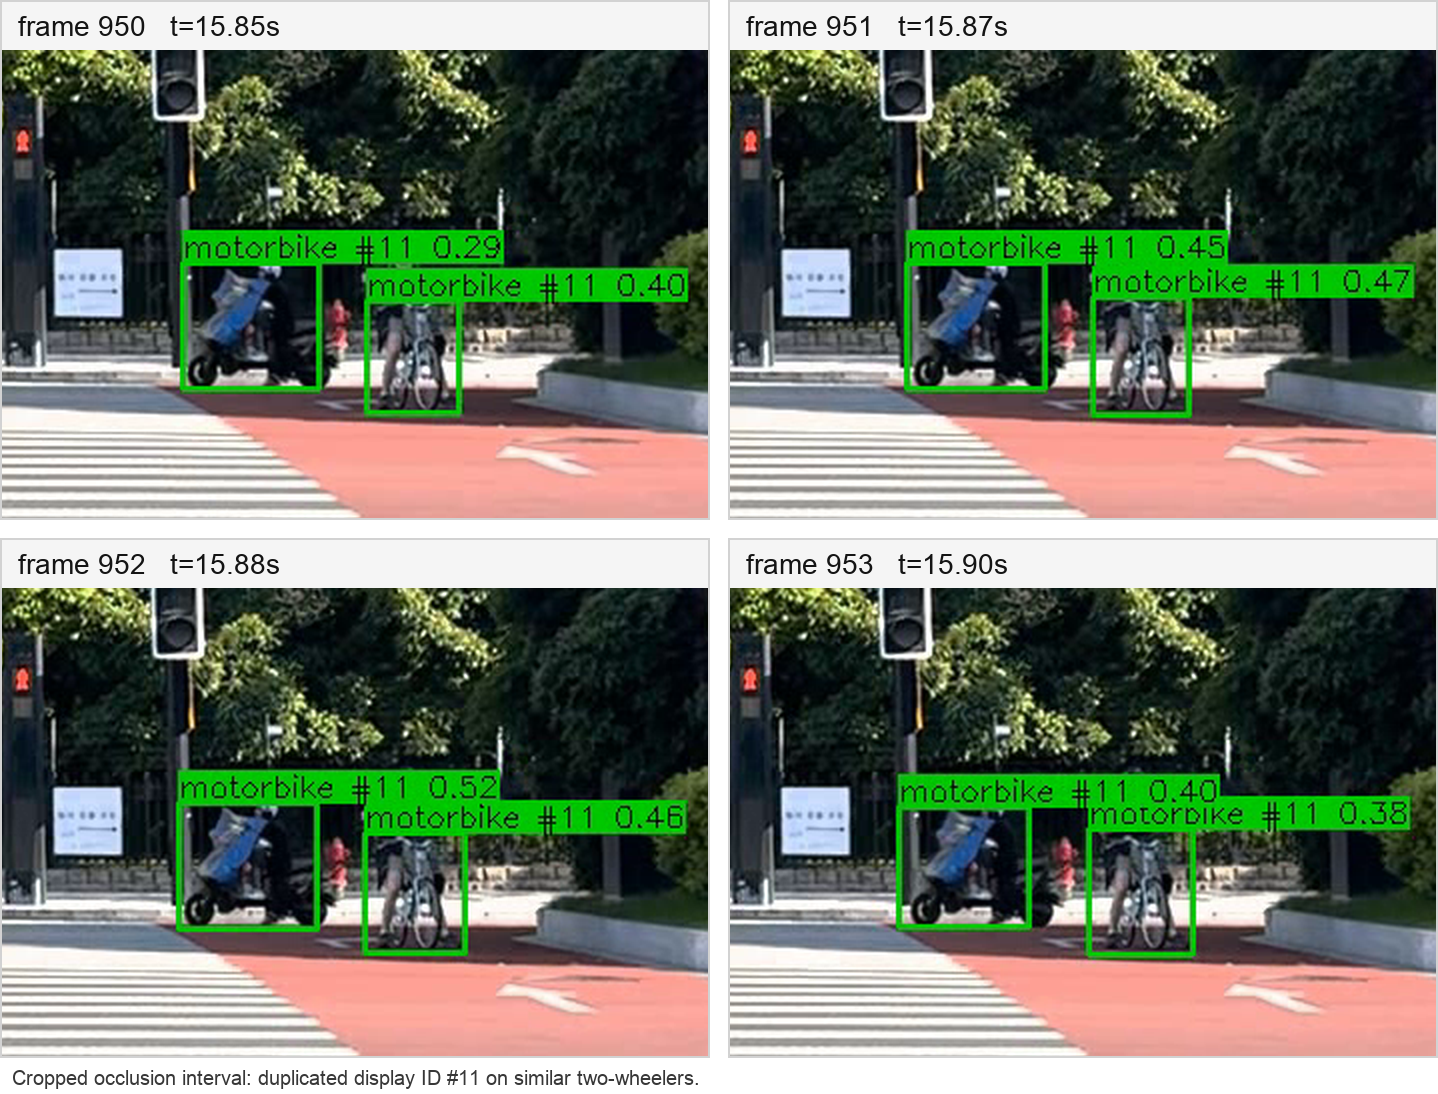
\includegraphics[width=0.94\textwidth]{task2_occlusion_id_jump_crop.png}
\caption{Task 2 遮挡片段裁剪图。frame 950--953 中两辆相似二轮车被错误映射到同一个 display id \texttt{\#11}。}
\label{fig:task2-occlusion}
\end{figure}

这一问题主要来自轨迹关联，而不是单帧检测。ByteTrack 依赖检测框位置、运动预测和置信度进行匹配，本身不显式使用外观 ReID 特征。当两个同类小目标短时间内距离很近，且检测框大小和运动方向相似时，卡尔曼预测和 IoU 匹配很难可靠地区分身份。后处理阶段为了减少 ID 断裂，又会根据类别族、预测位置和框尺寸把新 raw id 接回旧 display id；在该片段中，重连条件对相似二轮车过于宽松，使两个同时存在的目标共享了同一个 display id。

针对这类失败案例，后处理逻辑已经加入更保守的同帧保护：如果旧 raw id 仍在当前帧出现，就不再把另一个 raw id 接到同一个 display id 上。该规则用于降低同一帧内的 display id 复用风险，但图 \ref{fig:task2-occlusion} 仍表明，仅依赖几何位置、框尺寸和短时运动信息，不能从根本上解决遮挡后的身份恢复问题。若要进一步提升 ID 稳定性，需要引入外观 ReID 特征、相机运动补偿或更强的多目标跟踪器。

\subsection{Task 2 小结}

Task 2 最终得到一套基于 Road Vehicle 数据集微调的 YOLOv8s 检测权重，验证集 mAP50 为 0.5150。结合 ByteTrack 和 display id 后处理后，系统能够在测试视频中输出类别、检测框、跟踪 ID 和越线总数，30 fps 与 60 fps 两个版本分别统计到 19 与 25 次越线。主要不足集中在小目标、遮挡和相似目标密集交汇场景；frame 950--953 的例子表明，几何和运动信息足以改善部分漏计数，但在没有外观 ReID 的情况下仍可能发生 ID merge。

\section{Task 3：从零搭建 U-Net 与 Dice Loss 的语义分割}

\subsection{任务要求与数据口径}

Task 3 要求不使用任何预训练权重，从深度学习框架基础 API 手写 U-Net，包含完整下采样编码器、上采样解码器与 skip connection，并手写 Dice Loss。数据集为 Stanford Background Dataset，需要分别使用 Cross-Entropy、Dice Loss 和 CE+Dice 训练并比较验证集 mIoU。

实现位于 \texttt{hw2/task3/}。数据集中共有 715 张图像与对应 \texttt{.regions.txt} 标签，固定 seed=42 划分为 train 572 / val 143。标签包含 8 个语义类：sky、tree、road、grass、water、building、mountain、foreground object；原始 unknown 标签 $-1$ 映射为 ignore index 255，不参与 loss、pixel accuracy、mIoU 和 per-class IoU。

\subsection{U-Net 结构与 Dice Loss}

基础网络由四级 encoder、bottleneck、四级 decoder 和 $1\times1$ 输出卷积组成。每级编码块为两层 Conv-BatchNorm-ReLU，downsampling 使用 max pooling，upsampling 使用转置卷积或双线性上采样，随后与对应 encoder 特征拼接。最终优化中的 Attention U-Net 在 skip connection 前加入 additive attention gate，用 decoder gate feature 过滤 encoder skip feature。

Dice Loss 使用 softmax 概率和 one-hot 标签计算，并先用 ignore mask 去除 unknown 像素。对第 $c$ 类，其 soft Dice 写为
\[
D_c=\frac{2\sum_i p_{ic}y_{ic}+\epsilon}{\sum_i p_{ic}+\sum_i y_{ic}+\epsilon},
\]
整体 Dice Loss 为 $1-\frac{1}{C}\sum_c D_c$。组合损失为
\[
\mathcal{L}=\mathcal{L}_{CE}+\mathcal{L}_{Dice}.
\]
验证 mIoU 对每个非 ignore 类分别计算 $\mathrm{IoU}_c=\frac{TP_c}{TP_c+FP_c+FN_c}$，再对 8 个语义类取平均；unknown 像素不进入混淆矩阵和 mIoU 统计。

\begin{table}[!htbp]
\centering
\small
\caption{Task 3 数据与训练配置}
\label{tab:task3-config}
\begin{tabular}{@{}L{0.30\linewidth}L{0.56\linewidth}@{}}
\toprule
项目 & 配置 \\
\midrule
数据集 & Stanford Background Dataset \\
样本划分 & train 572 / val 143，固定 seed=42 \\
类别数 & 8 类；unknown 像素 ignore \\
基础输入尺寸 & $240\times320$；优化实验使用 $256\times320$ \\
基础模型 & 从零手写 U-Net，base channels 32 \\
最终模型 & 从零手写 Attention U-Net，base channels 64 \\
选模指标 & validation mIoU \\
最终评估增强 & horizontal-flip TTA + multi-scale TTA $[0.6,0.8,1.0,1.2,1.4]$ \\
优化器与学习率 & AdamW + cosine scheduler；基础实验 lr $3\times10^{-4}$，最终实验 lr $2\times10^{-4}$ \\
Batch size 与训练轮数 & 基础实验 batch size 8 / 80 epochs；最终实验 batch size 4 / 130 epochs \\
数据增强 & horizontal flip、color jitter、random scale crop；所有模型均从零训练 \\
\bottomrule
\end{tabular}
\end{table}

\subsection{三组损失函数对比}

表 \ref{tab:task3-loss} 为作业要求的三组基础实验。CE、Dice 和 CE+Dice 的 mIoU 非常接近，其中 CE+Dice 在单次实验中以 0.648970 略优。结合 per-class IoU，Dice-only 在 mountain 类上更好，但整体 pixel accuracy 略低；CE+Dice 在 sky、tree、grass、water、building 等主要类别上更均衡，因此作为后续优化基础。

\begin{table}[!htbp]
\centering
\small
\caption{Task 3 基础 loss 对比}
\label{tab:task3-loss}
\begin{tabular}{@{}L{0.30\linewidth}L{0.28\linewidth}S[table-format=3.0]S[table-format=1.6]S[table-format=1.6]@{}}
\toprule
实验 & 损失函数 & {Best epoch} & {Val mIoU} & {Val pixel acc} \\
\midrule
\texttt{task3\_unet\_ce} & Cross-Entropy & 69 & 0.648151 & 0.833211 \\
\texttt{task3\_unet\_dice} & 手写 Dice Loss & 63 & 0.648211 & 0.829996 \\
\texttt{task3\_unet\_ce\_dice} & CE + Dice & 52 & 0.648970 & 0.834739 \\
\bottomrule
\end{tabular}
\end{table}

\begin{figure}[!htbp]
\centering
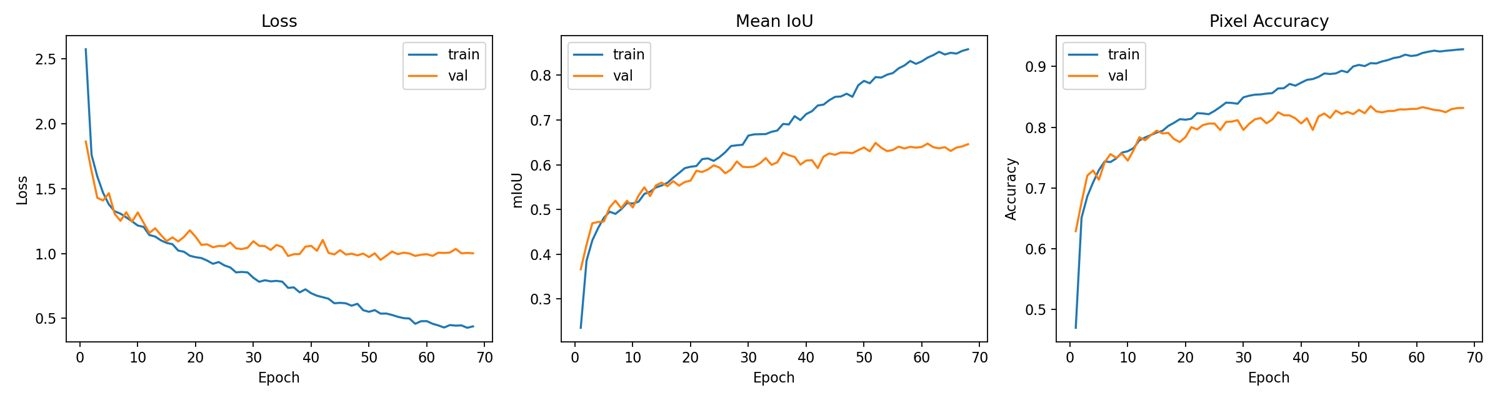
\includegraphics[width=0.90\textwidth]{task3_ce_dice_curves.jpg}
\caption{Task 3 CE+Dice 基础实验曲线。训练过程中记录 loss、mIoU 和 pixel accuracy。}
\label{fig:task3-base-curves}
\end{figure}

\subsection{进一步优化与最终模型}

在不违反作业约束的前提下，后续优化只修改从零训练的 U-Net 家族结构、输入尺寸、数据增强和评估增强。第一轮优化将 base channels 扩大到 64、输入调整到 $256\times320$，并加入 dropout 和 horizontal-flip TTA，使 mIoU 从 0.648970 提升到 0.665089。进一步加入 Attention Gate 后，plain Attention U-Net 达到 0.667801；再加入 random scale crop 和多 seed 尝试后，最终选择 seed=7 的 Attention U-Net checkpoint，并用多尺度 TTA 得到 0.701053。需要注意，Stanford Background 当前实验只使用固定 train/val 划分，因此最终结果是 validation mIoU，而不是独立测试集指标；多尺度 TTA 也在该验证协议下选择。

\begin{table}[H]
\centering
\small
\caption{Task 3 关键优化链路}
\label{tab:task3-optim}
\begin{tabular}{@{}L{0.34\linewidth}L{0.34\linewidth}S[table-format=1.6]S[table-format=1.6]@{}}
\toprule
实验 & 关键变化 & {Val mIoU} & {Val pixel acc} \\
\midrule
\texttt{task3\_unet\_ce\_dice} & 基础 U-Net + CE+Dice & 0.648970 & 0.834739 \\
\texttt{task3\_unet\_ce\_dice\_b64\_tta} & base=64，$256\times320$，dropout，flip TTA & 0.665089 & 0.842011 \\
\texttt{task3\_attention\_unet\_b64\_tta} & 加入 Attention Gate & 0.667801 & 0.843214 \\
\makecell[l]{\texttt{task3\_attention\_unet}\\\texttt{b64\_aug\_seed7\_tta}} & random scale crop，seed=7 & 0.695953 & 0.859910 \\
最终多尺度复评 & flip + multi-scale TTA & 0.701053 & 0.864931 \\
\bottomrule
\end{tabular}
\end{table}

\begin{figure}[H]
\centering
\begin{subfigure}{0.86\textwidth}
  \centering
  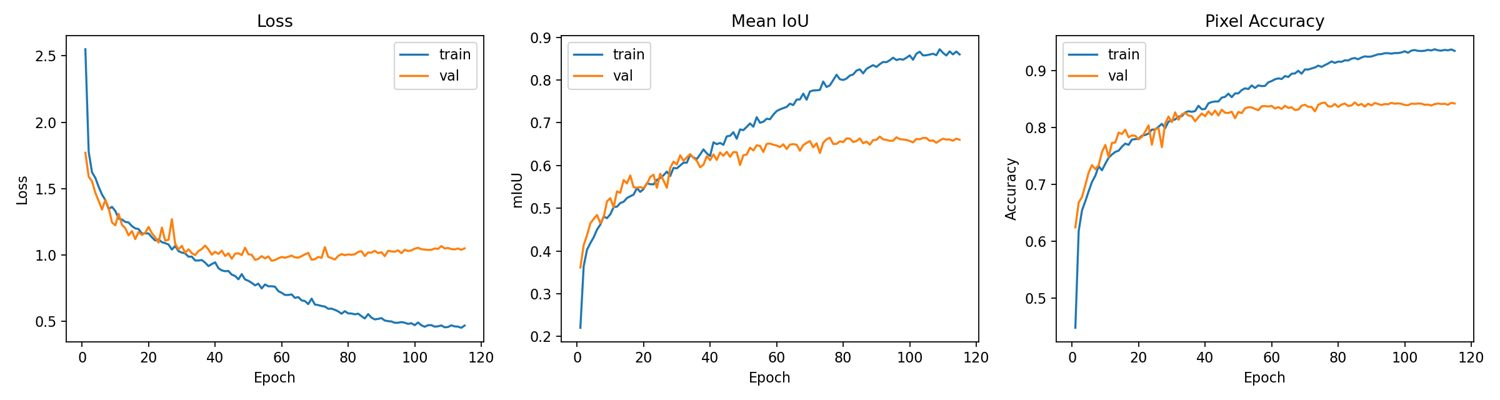
\includegraphics[width=\linewidth]{task3_attention_curves.jpg}
  \caption{Attention U-Net 结构优化}
\end{subfigure}
\vspace{2pt}

\begin{subfigure}{0.86\textwidth}
  \centering
  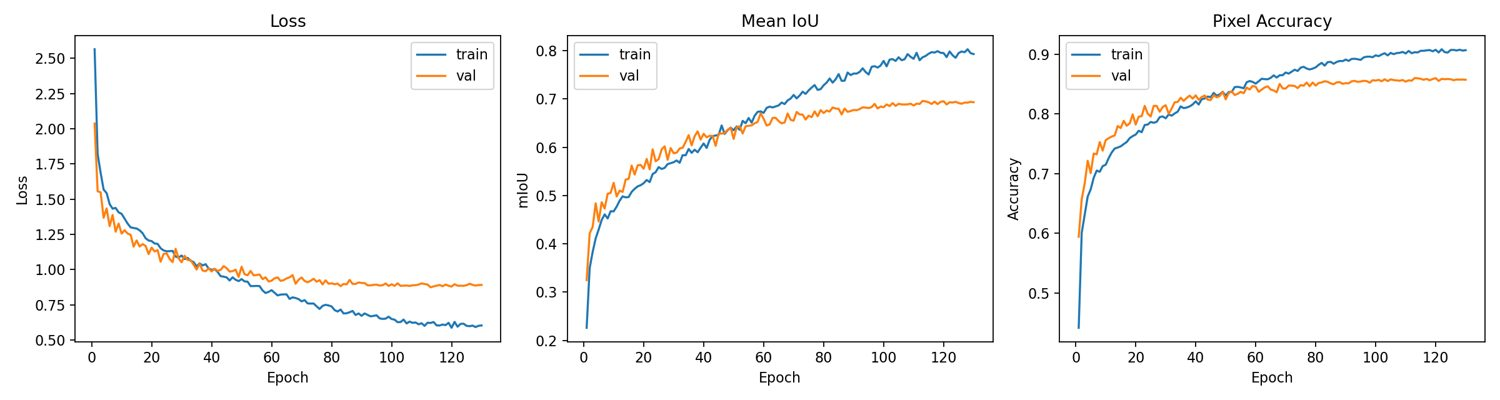
\includegraphics[width=\linewidth]{task3_final_curves.jpg}
  \caption{最终模型曲线}
\end{subfigure}
\caption{Task 3 代表性 SwanLab 曲线。}
\label{fig:task3-optim-curves}
\end{figure}

图 \ref{fig:task3-samples} 中，sky、road、building 等大面积区域通常较稳定，边界和小目标仍更容易出现误分割；mountain 类在最终 per-class IoU 中仍偏低，主要与样本占比小、外观和 tree/building/foreground object 混淆有关。

\begin{table}[H]
\centering
\small
\caption{Task 3 最终模型 per-class IoU}
\label{tab:task3-final-per-class}
\begin{tabular}{@{}L{0.30\linewidth}S[table-format=1.6]L{0.30\linewidth}S[table-format=1.6]@{}}
\toprule
类别 & {IoU} & 类别 & {IoU} \\
\midrule
sky & 0.904431 & water & 0.738596 \\
tree & 0.711124 & building & 0.759705 \\
road & 0.839109 & mountain & 0.249698 \\
grass & 0.764386 & foreground object & 0.641374 \\
\bottomrule
\end{tabular}
\end{table}

\begin{figure}[!t]
\centering
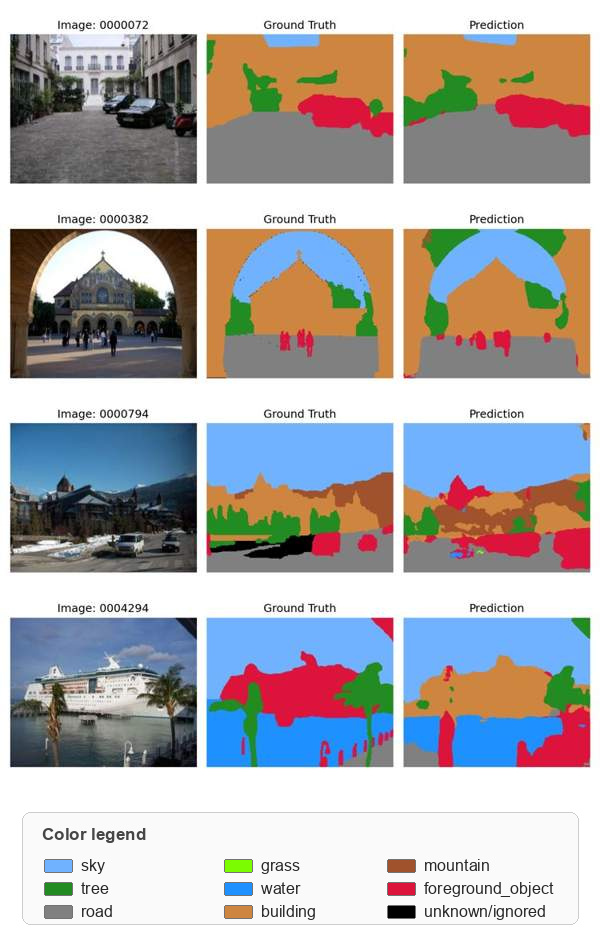
\includegraphics[width=0.68\textwidth]{task3_final_samples_with_legend.jpg}
\caption{最终 Attention U-Net 在验证集上的分割样例与类别颜色图例。}
\label{fig:task3-samples}
\end{figure}
\FloatBarrier
\enlargethispage{3\baselineskip}

\subsection{mIoU 0.75 目标优化尝试与约束分析}

围绕 mIoU 0.75 目标，进一步尝试了 U-Net++、scSE、ASPP bridge、deep supervision、Lovasz-Softmax、更高分辨率和更大 batch。所有模型仍从零训练，没有使用 SAM、DeepLab、SegFormer、torchvision segmentation models、外部数据或预训练权重。最好尝试为 \texttt{task3\_unetpp\_b64\_384\_lovasz\_ds\_tta}，多尺度复评约为 0.6953，低于最终推荐模型。因此，在当前 \texttt{hw2.md} 约束下，继续堆高分辨率或更复杂从零结构并没有带来接近 0.75 的收益；若要显著突破，可能需要预训练 backbone、外部数据、现成强分割模型或 ensemble，但这些超出当前作业约束，因此未采用。

\section{结论}

Task 1 已完整覆盖 baseline、超参数分析、预训练消融和注意力结构对比；最终额外优化模型 ConvNeXt-Tiny 在测试集上达到 96.08\%。Task 2 已按 hw2.md 要求完成 Road Vehicle 数据集上的 YOLOv8s 专属检测模型训练、交通视频逐帧检测与多目标跟踪、遮挡片段 ID 跳变分析和基于虚拟线的越线计数；检测模型最佳 mAP50 为 0.5150，两个视频版本的最终计数分别为 19 与 25。Task 3 已完整覆盖从零手写 U-Net、手写 Dice Loss 和三组 loss 对比；最终在严格不使用预训练和现成分割模型的约束下达到 validation mIoU 70.1053\%。

\end{document}
